\documentclass{beamer} %twoside
\usetheme{Madrid}
%\usepackage[left=2cm,right=2cm,top=2cm,bottom=3cm]{geometry}
%\usepackage{fontspec}
%\setmonofont{FreeMono}
%\usepackage[utf8]{inputenc}
%\usepackage{amsmath}
%\usepackage{amssymb}
%\usepackage{amsfonts}
\usepackage{hyperref}
%\usepackage{makecell}
%\usepackage{xcolor}
%\usepackage{xspace}
%\usepackage[english]{babel}
%\usepackage{underscore}
%\usepackage{listings}
%\usepackage{pygmentex}
%\usepackage{minted}
%\usepackage{newunicodechar}
%\usepackage{setspace}
%\usepackage{comment}
%\usepackage{enumitem}
%\usepackage{tcolorbox}
%\usepackage{tikz-inet}
\usepackage{graphicx}
%\graphicspath{ {./padic-L-functions/PadicLFunctions4/} }
%\usetikzlibrary{positioning}
%\usepackage[numbers]{natbib}
%\usemintedstyle{tango}
%\def\lstlanguagefiles{lstlean.tex}
%\lstset{language=lean}
\bibliographystyle{plainurl}

%\addtolength{\oddsidemargin}{-.875in}
%\addtolength{\evensidemargin}{-.875in}
%\addtolength{\textwidth}{1.75in}
%\onehalfspacing
%\doublespacing

%\newtheorem{theorem}{Theorem}
%\newtheorem{definition}{Definition}[chapter]
%\newtheorem{theorem}{Theorem}[chapter]

\definecolor{keywordcolor}{rgb}{0.7, 0.1, 0.1}   % red
\definecolor{commentcolor}{rgb}{0.4, 0.4, 0.4}   % grey
\definecolor{symbolcolor}{rgb}{0.4, 0.4, 0.4}    % grey
\definecolor{sortcolor}{rgb}{0.1, 0.5, 0.1}      % green

%\newcommand{\C}{\mathbb{C}}
%\newcommand{\lean}[1]{\texttt{#1}\xspace} % for writing Lean expressions
%\newcommand*{\OK}[1][K]{\mathcal{O}_{#1}}
%\newcommand*{\Cl}{\mathcal{C}\kern-.075em l}
% \DeclareMathOperator{\Cl}{Cl}
%\newcommand*{\Fq}[1][q]{\mathbb{F}_{#1}}
%\DeclareMathOperator{\Tr}{Tr}
%\newcommand{\mathlib}{\textsf{mathlib}\xspace}
%\newcommand{\N}{\mathbb{N}}
%\newcommand{\R}{\mathbb{R}}
%\newcommand{\pow}{\textasciicircum\xspace}
%\newcommand{\Q}{\mathbb{Q}}
% \newcommand{\Qbar}{\mathbb{\bar{Q}}}
%\newcommand{\Z}{\mathbb{Z}}
%\DeclareMathOperator{\Frac}{Frac}

%\newunicodechar{^}{\ensuremath{\textasciicircum}}

\renewcommand\UrlFont{\color{blue}\rmfamily}

%\title{formalisation of $p$-adic $L$-functions}
%\author{Ashvni Narayanan}

%\input{blocked.sty}
%\input{uhead.sty}
%\input{boxit.sty}
%\input{icthesis.sty}

\title{Lean and LeanAIde}
\author{Ashvni Narayanan}
\institute{Sydney Mathematical Research Institute}

\begin{document}
\frame{\titlepage}

\begin{frame}
\frametitle{Table of Contents}\pause
\begin{itemize}
\item[\textbullet] What is formalisation? \pause
\item[\textbullet] What is Lean? \pause
\item[\textbullet] Formalisation of number theory in Lean \pause
\item[\textbullet] What is autoformalisation? \pause
\item[\textbullet] What is LeanAIde? \pause
\end{itemize}
\end{frame}

\begin{frame}
\frametitle{Some stories}
\begin{itemize}
    \item [\textbullet] Wikipedia : ``Augustin Louis Cauchy in 1821 published a faulty proof of the false statement that the pointwise limit of a sequence of continuous functions is always continuous. Joseph Fourier and Niels Henrik Abel found counter examples in the context of Fourier series. Dirichlet then analyzed Cauchy's proof and found the mistake: the notion of pointwise convergence had to be replaced by uniform convergence." \pause
    \item [\textbullet] In 1937, a German-Jewish mathematician Samuel I. Krieger once claimed to have found a counterexample to Fermat's last theorem : $x^n + y^n = z^n$, for $x = 1324$, $y = 731$, and $z = 1961$. Note that the LHS can only end in 5 or 7, while the RHS can end in 1. \pause
    \item [\textbullet] Chapter 3, What is Mathematics, Really? : ``Newton found the speed of a falling stone by dividing 0/0. Berkeley called him to account for bad algebra, but admitted Newton had the right answer... Mistake or not?"
\end{itemize}
\end{frame}
\begin{frame}
\frametitle{Some stories}
Excerpt from What is Mathematics, Really? \pause
\begin{center}
Henri Poincaré said it was strange that mistakes happen in mathematics, since mathematics is just sound reasoning, such as anyone in his right mind follows. His explanation was memory lapse—there are only so many things we can keep in mind at once. .. \pause Some mistakes come from keeping old assumptions in a new context. .. \pause We mathematicians make mistakes, even important ones, even in famous papers that have been around for years.
\end{center}
\end{frame}
\begin{frame}
\frametitle{Some stories}
Excerpt from What is Mathematics, Really?
\begin{center}
Can we be sure that we, unlike our predecessors, are not overlooking big gaps?
\end{center}    
\end{frame}
\begin{frame}
\frametitle{The question}
\begin{center}
Can we find a reliable and uniform system to validate the precision of the mathematics we create?
\end{center}
\end{frame}
\begin{frame}
\frametitle{Enter formalisation}
\begin{center}
``Formal verification involves the use of logical and computational methods to establish claims that are expressed in precise mathematical terms."  
\end{center}
(Theorem Proving in Lean) \pause \newline
There are several proof assistants for formal proof verification, such as Isabelle, Coq, Lean etc. \pause \newline 
We use Lean 3, an interactive theorem prover.
%, which is based on dependent type theory. \pause \newline 
%It has a mathematical library called \texttt{mathlib}, which is being built by computer scientists and mathematicians since 2017. \pause \newline
%\texttt{mathlib} contains 112601 theorems, including those which are taught in undergraduate courses. \pause \newline
%It also contains many advanced topics such as condensed mathematics, perfectoid spaces, a solution to the continuum hypothesis etc.
\end{frame}
\begin{frame}
\frametitle{What is Lean?}
\begin{itemize}
\item[\textbullet] Lean is an interactive theorem prover. \pause
\item[\textbullet] It is being used by several mathematicians to \textit{formally verify} theorems and store 
them in an online library called \texttt{mathlib}. \pause
%\item[\textbullet] A fundamental feature is Lean’s \textit{typeclass inference} system, which ``remembers'' properties. \pause
\item[\textbullet] We use \texttt{mathlib}, which contains 112601 theorems, with over 300 contributors. 
It is impossible to isolate and cite their work individually. We extend our thanks to all. \pause
\item[\textbullet] The guiding spirit of \texttt{mathlib} is to prove theorems in the highest possible generality. \pause
\item[\textbullet] \texttt{mathlib} uses type theory as a building block, instead of set theory, which leads to subtle 
(but consequential) differences in proofs on paper and in Lean. 
\end{itemize}
\end{frame}
\begin{frame}
\frametitle{A little bit about type theory}
\begin{itemize}
\item [\textbullet] Every element has a unique type. For example, \texttt{1 : Nat} represents 1 of type naturals. \pause
\item [\textbullet] This is different from \texttt{1 : Rat}, 1 of type rationals. \pause
\item [\textbullet] How do we identify the two? We use the canonical map $\mathbb{N} \to \mathbb{Q}$, which takes \texttt{1 : Nat} to \texttt{1 : Rat}. \pause
\item [\textbullet] The type of propositions, \texttt{Prop}, is special : a term of type a proposition \texttt{p} is a proof of it. \pause
\item [\textbullet] Lean does not remember the proof, just its existence.
\item [\textbullet] Let us take a look at an example.
\end{itemize}
\end{frame}
\begin{frame}
\frametitle{Some theories that have been formalized in Lean}
\begin{itemize}
\item [\textbullet] Broadly all undergraduate math curricula
\item [\textbullet] Perfectoid spaces (Kevin Buzzard, Johan Commelin, Patrick Massot, 2020)
\item [\textbullet] Gardam's disproof of the unit conjecture (Siddhartha Gadgil, Anand Rao Tadipatri, 2022)
\item [\textbullet] Condensed mathematics (Johan Commelin et al, 2022)
\item [\textbullet] Independence of the continuum hypothesis (Jesse Han, Floris van Doorn)
\item [\textbullet] Existence of sphere eversions (Patrick Massot, Floris van Doorn, Oliver Nash, 2021)
\end{itemize}
\end{frame}
\begin{frame}
\frametitle{Some number theory results that have been formalized in Lean}
\begin{itemize}
\item [\textbullet] Quadratic reciprocity (Michael Stoll)
\item [\textbullet] Pell's equation and Matiyasevic's theorem (Mario Carneiro, Michael Stoll)
\item [\textbullet] Hensel's lemma on $\mathbb{Z}_p$ (Rob Lewis)
\item [\textbullet] Finiteness of the class number (Anne Baanen, Sander Dahmen, Filippo Nuccio, A.N.)
\item [\textbullet] Dirichlet's Unit Theorem (Xavier Roblot)
\item [\textbullet] Adéles and idéles (María Inés de Frutos-Fernández, 2022)
\item [\textbullet] Local fields and class field theory (María Inés de Frutos-Fernández, Filippo A.E. Nuccio et al)
\item [\textbullet] $p$-adic $L$-functions (A.N.)
\item [\textbullet] Fermat's last theorem? (Kevin Buzzard et al.)
\end{itemize}
\end{frame}
\begin{frame}
\frametitle{What are $p$-adic $L$-functions?}
Kummer's congruence states that, when $h$ and $k$ are positive even integers not divisible by $p - 1$ :
$$ \frac{B_h}{h} \equiv \frac{B_k}{k} (\texttt{mod }p) $$
for the Bernoulli numbers $B_h$ and $B_k$.
Kubota and Leopoldt's search for a meromorphic function that helps study this congruence led them to the $p$-adic $L$-function. 
%They play an important role in Iwasawa theory, since they give information regarding $p$-adic class numbers. 
They are characterized by their values at negative integers,
$$ L_p (1 - n, \chi) = -(1 - \chi \omega^{-n}(p)p^{n - 1}) \frac{B_{n, \chi \omega^{-n}}}{n} $$  
for $n > 1$. \\
We are going to define $p$-adic $L$-functions in terms of a $p$-adic integral.
\end{frame}

\begin{frame}[fragile]\label{padicdef}
\frametitle{Definition of $p$-adic $L$-function}
\begin{center}

\includegraphics[width=\textwidth]{./padic-L-functions/PadicLFunctions4/paLfdef}
\end{center}
\end{frame}

\begin{frame}[fragile]\label{dircharsec}
\raggedbottom{\hyperlink{padicdef}{\beamerbutton{Back}}}
\frametitle{Dirichlet characters}
\begin{itemize}
\item[\textbullet] A Dirichlet character is generally a multiplicative group homomorphism into $\mathbb{C}$. \pause
\item[\textbullet] We define a Dirichlet character of level $n$ to be a monoid homomorphism $\mathbb{Z} / n \mathbb{Z}^{\times} \to R^{\times}$, where $R$ is a monoid. This is a function on $\mathbb{Z}$ when $n = 0$ : \pause
\end{itemize}
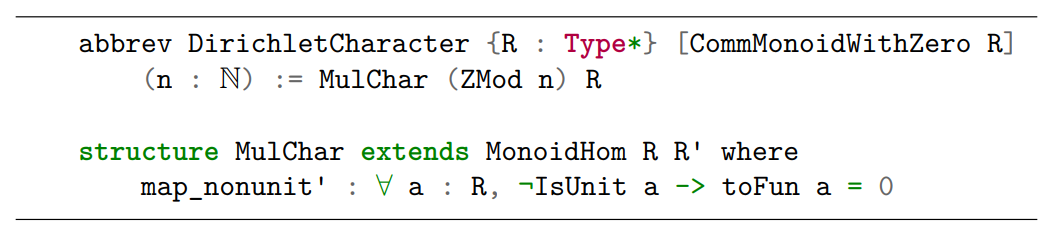
\includegraphics[width=\textwidth]{DirChardef}
\end{frame}

\begin{frame}[fragile]
\frametitle{$p$-adic measures}
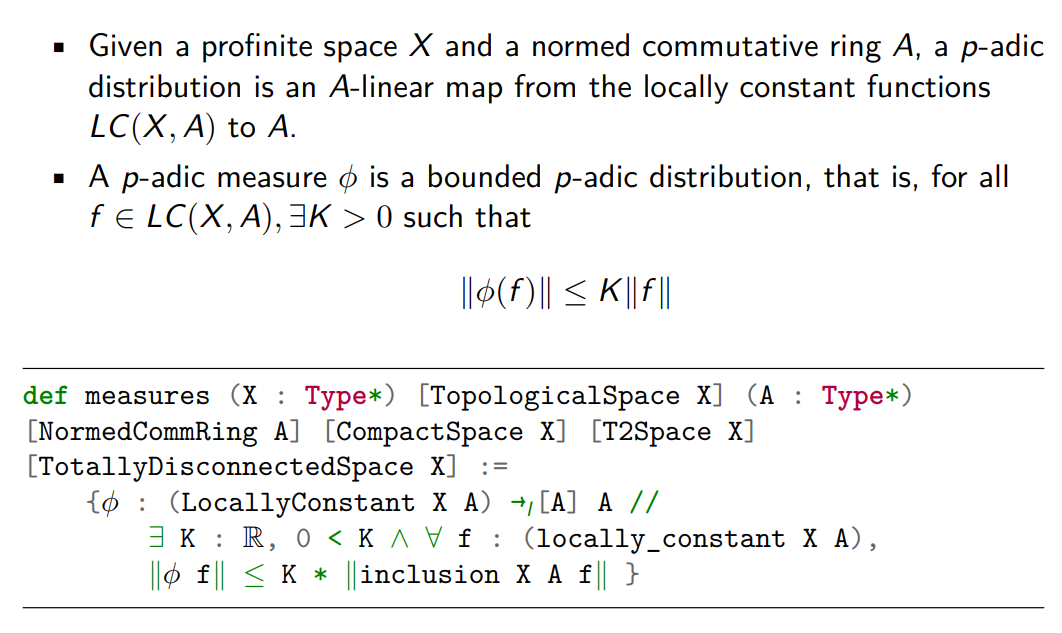
\includegraphics[width=\textwidth]{padicmeasure}
\end{frame}

\begin{frame}[fragile]
\frametitle{$p$-adic integral}
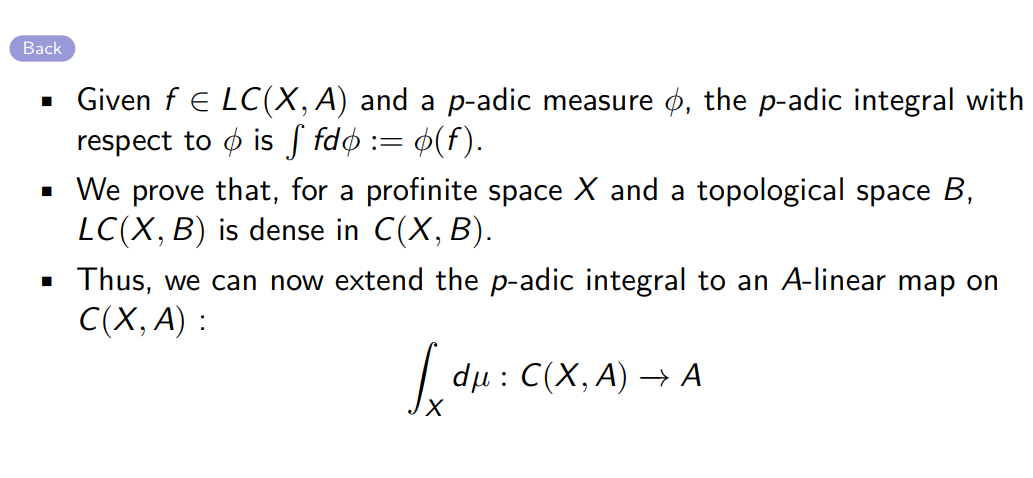
\includegraphics[width=\textwidth]{padicintegral}
\end{frame}
    
\begin{frame}[fragile]
\frametitle{$p$-adic integral}
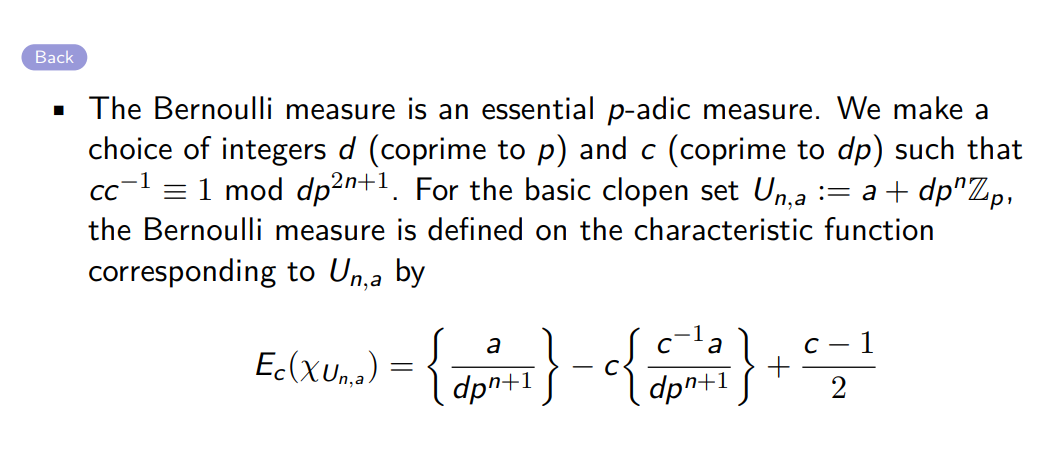
\includegraphics[width=\textwidth]{bermeas}
\end{frame}

\begin{frame}[fragile]
\frametitle{Is this what we want?}
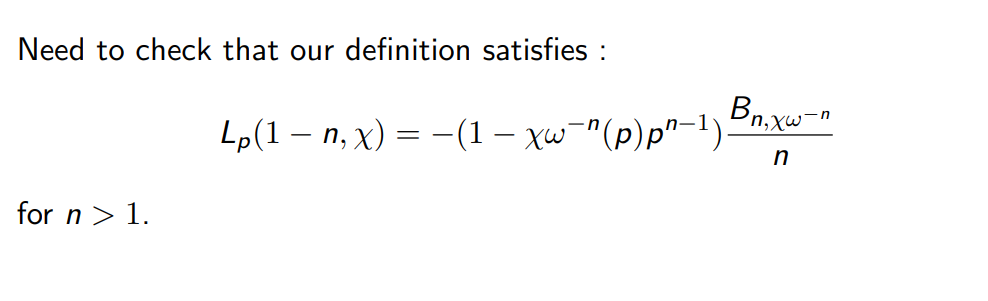
\includegraphics[width=\textwidth]{isthis}
\end{frame}

\begin{frame}[fragile]
\frametitle{A property of the generalized Bernoulli numbers}
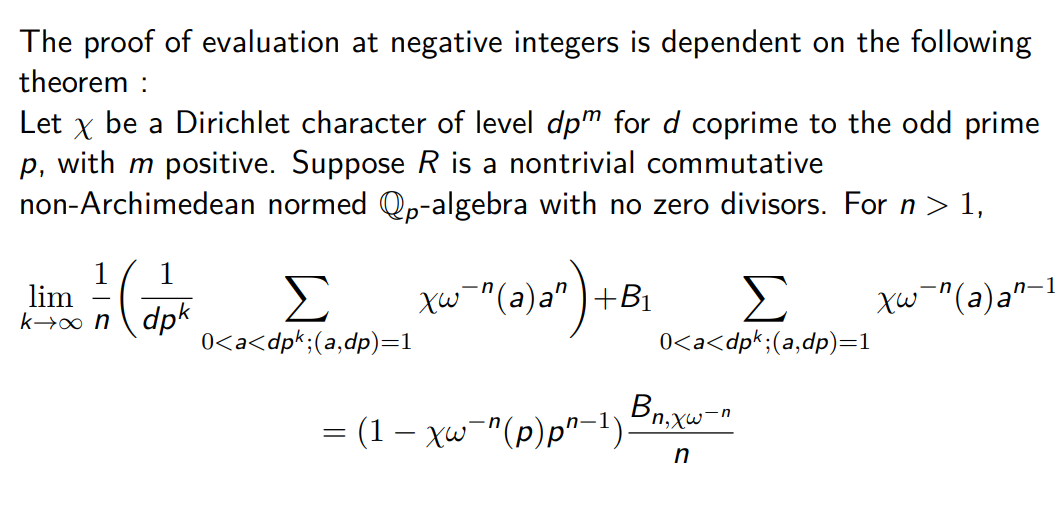
\includegraphics[width=\textwidth]{gbnprop}
\end{frame}

\begin{frame}[fragile]
\frametitle{Remarks}
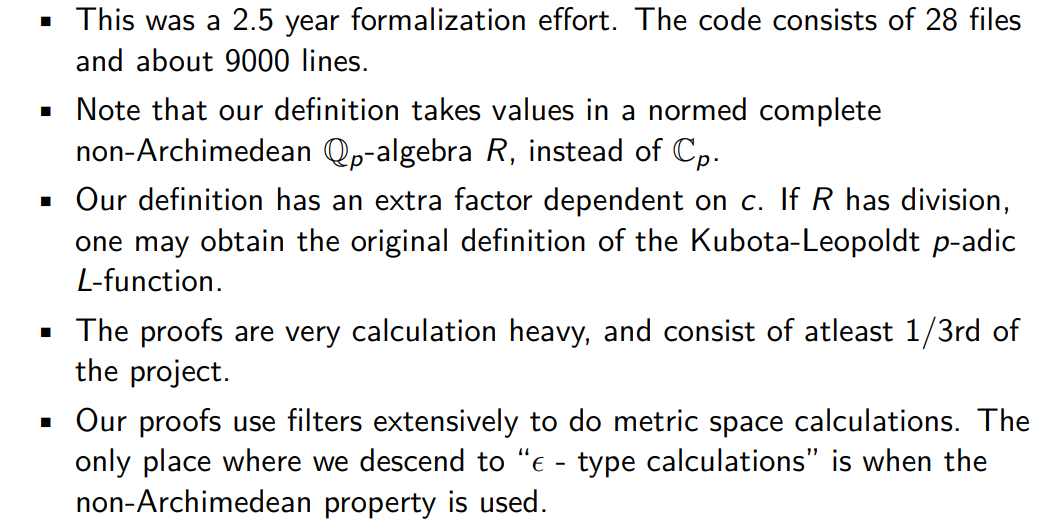
\includegraphics[width=\textwidth]{remarks}
\end{frame}

\begin{frame}[fragile]
\frametitle{Crude mind map}
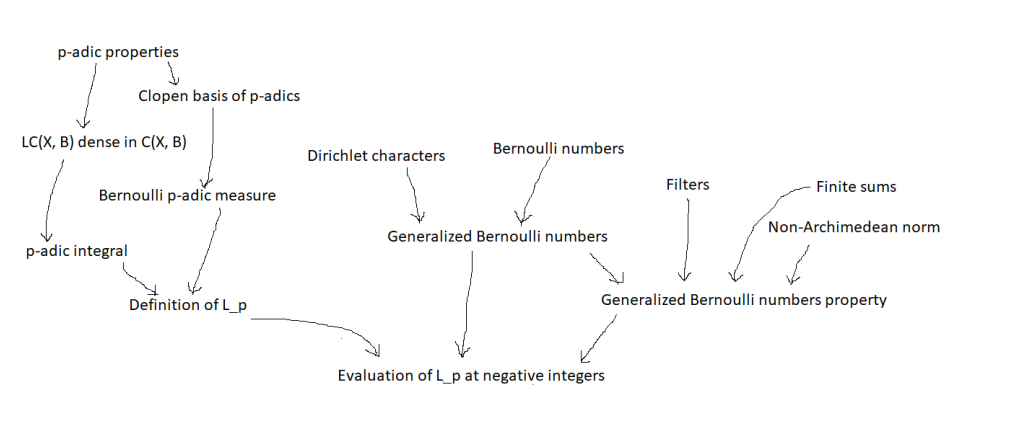
\includegraphics[width=\textwidth]{mindmap}
\end{frame}

\begin{frame}
The next part of this talk is born from the following paper :
\begin{center}
Towards a Mathematics Formalisation Assistant using Large Language Models
\end{center}
which is a joint work with Prof Siddharth Gadgil, Anand Rao Tadipatri, Ayush Agrawal, and Dr Navin Goyal.
\end{frame}
\begin{frame}
\frametitle{Why autoformalisation?}
\begin{itemize}
\item [\textbullet] One may not know what the names of the lemmas they require to prove their theorem, and if it is in the library. \pause
\item [\textbullet] They might have to run through several cases with similar (long) proofs. \pause
\item [\textbullet] They might have to prove several elementary lemmas, which might be ``obvious'' to the human mind. \pause
\end{itemize}
This could result in a difficult experience for the general mathematician who is looking to formalise their results easily and quickly. Autoformalisation aims to reduce the effort required to get results formally verified.
\end{frame}
\begin{frame}
\frametitle{What is LeanAIde?}
LeanAIde is an autoformalisation tool, which translates natural language mathematics into Lean code. \pause \newline
In particular, it takes as input `docstring - like statements' and suggests their translation. \pause \newline 
Let us take a look.
\end{frame}
\begin{frame}
\frametitle{How was LeanAIde built?}
\begin{itemize}
\item [\textbullet] A Large Language Model (LLM) is a deep learning algorithm which is trained on large datasets (typically around 1 billion parameters). It can be used for natural language processing tasks, such as prediction, translation etc. \pause
\item [\textbullet] LeanAIde uses a LLM called GPT 3.5-Turbo (initially Codex). Codex has been trained on 54 million public software repositories, including \texttt{mathlib}. \pause
\item [\textbullet] We tried translations of 3 kinds : short theorem statements, theorem proofs, and complex theorem statements. \pause
\item [\textbullet] Currently, LeanAIde offers suggestions or translations only for theorem statements.
\end{itemize}
\end{frame}
\begin{frame}
\frametitle{Short theorem statements : Prompt Engineering}
\begin{itemize}
\item [\textbullet] Codex takes as input a prompt. There are two kinds of prompts that were given to Codex : fixed and input dependent. \pause
\item [\textbullet] Input dependent prompts (IDP) are those which are dependent on the statement to be translated. From the statement, the generated prompts are docstrings (and associated theorems) from \texttt{mathlib} which are `similar' to the given statement. \pause
\item [\textbullet] There are two notions of similarity : keyword matching and sentence embedding proximity. \pause
\item [\textbullet] Fixed prompting (FP) is where a fixed set of prompts are provided as input to Codex, independent of the statement to be translated. \pause
\item [\textbullet] The idea of using input-dependent prompting for autoformalisation is a first.
\end{itemize}
\end{frame}
\begin{frame}[fragile]
\frametitle{Example of input-dependent prompting}
The given input : ``If a vector space has dimension ‘2‘ then it is finite dimensional.'' \pause \\
Input dependent prompts :
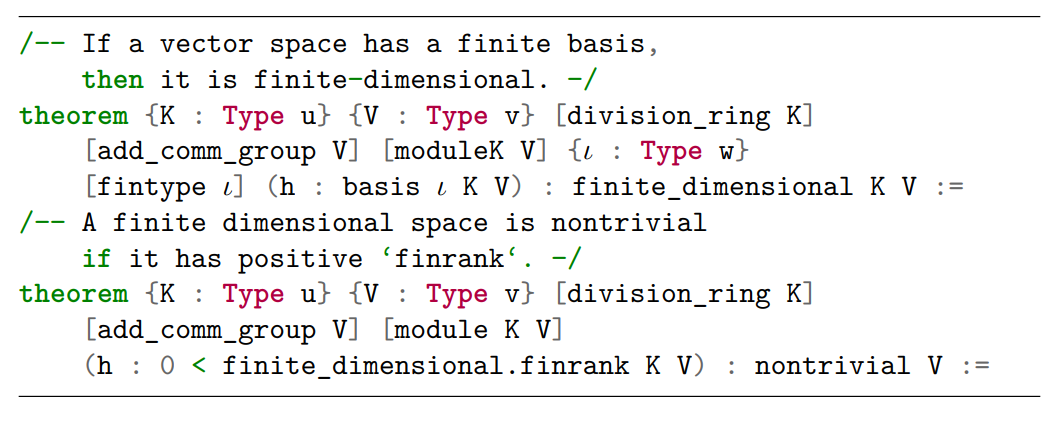
\includegraphics[width=\textwidth]{inputdep}
\end{frame}
\begin{frame}[fragile]
\frametitle{Example of input-dependent prompting}
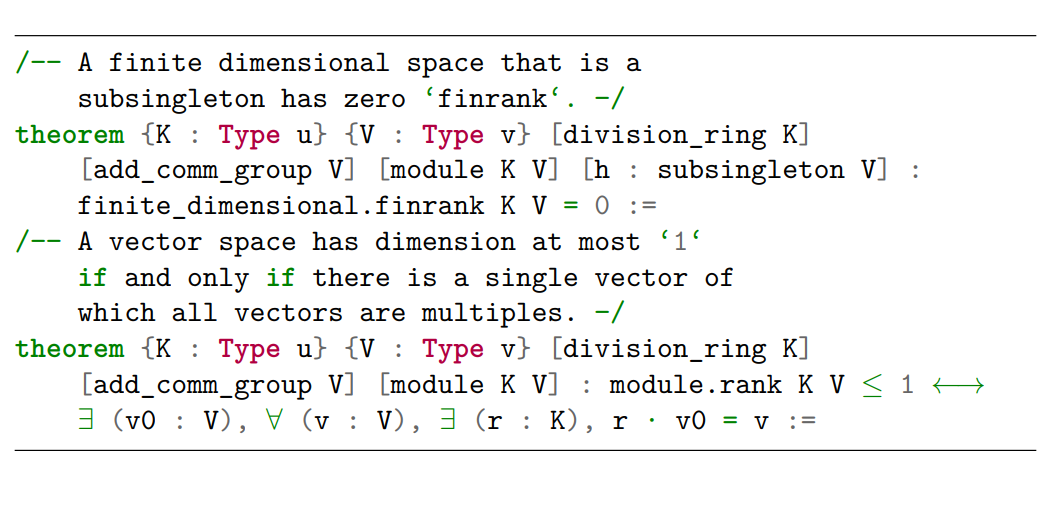
\includegraphics[width=\textwidth]{inputdep2}
\end{frame}
\begin{frame}[fragile]
\frametitle{Example of input-dependent prompting}
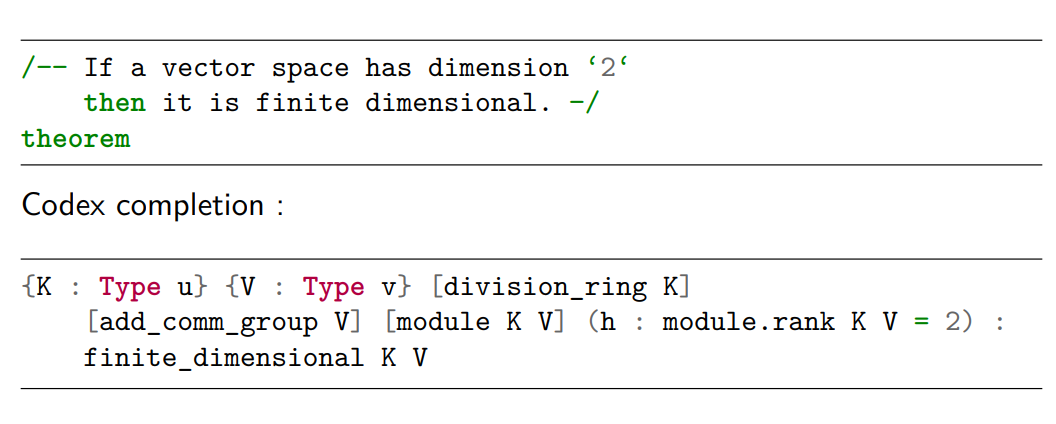
\includegraphics[width=\textwidth]{inputdep3}
\end{frame}
\begin{frame}
\frametitle{Short theorem statements : Post processing}
\begin{itemize}
\item [\textbullet] Given a statement, for each completion provided by Codex, we checked if the completion would `elaborate'. \pause
\item [\textbullet] This is similar (and stronger) to checking if the completions are type-correct. \pause
\item [\textbullet] This process confirms that the given output is valid Lean code (irrespective of whether it is accurate or not). \pause
\item [\textbullet] This method filters out statements which are incorrect, and is hence a good measure for accuracy.
\end{itemize}
\end{frame}
\begin{frame}
\frametitle{Short theorem statements : Evaluation dataset}
\begin{itemize}
\item [\textbullet] 120 theorem statements were evaluated. This dataset consists of undergraduate level statements. \pause
\item [\textbullet] This was further divided into 3 groups of 40 statements each : mathematical theorems, silly statements and false statements. \pause
\item [\textbullet] Each statement first went through prompt engineering and then post processing. \pause
\item [\textbullet] We conclude that, with careful input-dependent prompting and post processing, these statements could be formalised with nearly 75\% accuracy.
\end{itemize}
\end{frame}
\begin{frame}
\frametitle{Complex theorem statements}
\begin{itemize}
\item [\textbullet] We carried out a case study to evaluate performance of Codex with respect to translating complex mathematical statements. \pause
\item [\textbullet] Our examples are from undergraduate level Putnam competition and
involve complex formulas. \pause
\item [\textbullet] We evaluated 15 statements, with 6 outputs generated for each : 3 IDP and 3 FP. 
\end{itemize}
\end{frame}
\begin{frame}
\frametitle{Complex theorem statements : Results}
\begin{itemize}
\item [\textbullet]  Of the 90 evaluations, 1 was accurate, while 9 were almost entirely correct, and could be made completely accurate with minor modifications. \pause
\item [\textbullet] The main cause for this is two-fold : complex \LaTeX expressions, and complex English idioms, such as : ``... the intersection of every d + 1 of these sets ..''. \pause
\item [\textbullet] Our evaluations suggest that FP perform better for the former. \pause
\item [\textbullet] IDP outputs are formalised to a more abstract setting. This is clearly because they are from \texttt{mathlib}. \pause
\item [\textbullet] Our dataset, however, is too small to make a decisive conclusion.    
\end{itemize}
\end{frame}
\begin{frame}
\frametitle{Theorem proofs}
\begin{itemize}
\item [\textbullet] We aim for ``useful'' outputs, instead of complete formalised proofs. \pause
\item [\textbullet]  While in some cases a similar proof appears in \texttt{mathlib}, our results are not contaminated since the structure of our natural language proofs are significantly different. \pause
\item [\textbullet] Due to lack of aligned proofs, IDP is infeasible in this case. \pause
\item [\textbullet] We graded 3 different proof formats for 13 theorems. Their proofs are from various
sources such as ProofWiki, university courses etc., of varying proof technique, domain and difficulty
level.
\end{itemize}
\end{frame}
\begin{frame}
\frametitle{Theorem proofs : Theorems}
\begin{itemize}
\item [\textbullet] The absolute value function is convex 
\item [\textbullet] Symmetric real matrices have real eigenvalues
\item [\textbullet] Schur's lemma
\item [\textbullet] Schur's inequality
\item [\textbullet] $\mathbb{R}^n$ is paracompact
\item [\textbullet] Overflow theorem
\item [\textbullet] Density of irrational orbit
\item [\textbullet] Contraction mapping theorem
\item [\textbullet] The class number of a PID is 1
\item [\textbullet] A bipartite graph is two colorable
\item [\textbullet] $p$-adic units are coprime
\item [\textbullet] Nesbitt's inequality
\item [\textbullet] Evaluation of Bernoulli polynomials
\end{itemize}
\end{frame}
\begin{frame}
\frametitle{Theorem proofs : Proof formats}
\begin{itemize}
\item [\textbullet] Proof formats vary across two axes: the level of detail and whether the formal proof has comments. The following are the 3 proof formats : \pause
\item [\textbullet] Full proof : The complete proof as is. \pause
\item [\textbullet] Proof outline : Only the main steps of the proof are listed in order. A tool that is capable of producing good outlines could still be valuable to a user since one could, in principle, iteratively produce outlines of the main proof and all its steps, until one is left with trivial steps that can handled by automation. \pause
\item [\textbullet] Proof outline with premises : This format is at an intermediate level of detail; each proof step is listed along with a list of premises from which it can be deduced. This is done by introducing a fictitious new Lean tactic \texttt{auto} that takes as arguments the list of theorems that go into a proof along with an optional list of Lean tactics that may be helpful. \pause
\item [\textbullet] Each of these proof formats was used as is and with comments before each proof step.
\end{itemize}
\end{frame}
\begin{frame}[fragile]
\frametitle{Theorem proofs : Example}
\begin{figure}
    \includegraphics[width=\linewidth]{codex-proof-example.png}
\end{figure}
\end{frame}        
\begin{frame}
\frametitle{Theorem proofs : Results}
\begin{itemize}
\item [\textbullet] We graded each output from 0 to 4, depending on the accuracy of the output : 0 if the output does not help with formalising the complete proof; 1 if the
output slightly decreases the effort needed to formalise the complete proof; 2 if the output makes it
substantially easier to formalise the complete proof; 3 if the output only needs few minor corrections;
4 if the output is fully correct. \pause
\item [\textbullet] No completion received a perfect score of 4. For 8 of the 13 theorems, at least one Codex completion (out of 18), was marked 3. \pause
\item [\textbullet] The main sources of lower scores were errors related to incorrect
natural language statement translations that could be mathematically incorrect, irrelevant or invalid
Lean code. Some lower scores were also due to step repetitions and hallucinations. \pause
\item [\textbullet] Overall, we found that the generated proofs were well aligned with the natural language proofs and also well-structured as per Lean style. \pause
%\item [\textbullet] There were very few instances where the output proof formats deviated from the natural language proofs, and Codex merged proofs from different sources.
\end{itemize}
\end{frame}
\begin{frame}[fragile]
\frametitle{Theorem proofs : Results}
\begin{figure}
    \includegraphics[width=\linewidth]{chart-proof-autoformalization.png}
\end{figure}
\end{frame}
\begin{frame}
\frametitle{Related results}
\begin{itemize}
\item [\textbullet] LLM Step (Welleck, Sean and Saha, Rahul) : It is a Lean 4 tactic for suggesting proof steps using a language model. \pause
\item [\textbullet] Sagredo : Provides an automated dialogue between GPT and Lean. \pause
\item [\textbullet] Draft, Sketch and Prove (Albert Q. Jiang, et al) : Guides  a method that maps informal proofs to formal proof sketches. Guiding an automated prover with these sketches enhances its performance from 20.9\% to 39.3\% on a collection of mathematical competition problems.
\end{itemize}
\end{frame}
\begin{frame}
\frametitle{Conclusion}
Autoformalisation is a powerful and useful tool that can help the general mathematician with verifying their results in a speedy and efficient manner. \\ 
It is currently able to formalise short theorem statements very well. \\
Soon, it should be able to formalise complex statements and proofs as well.
\end{frame}
\begin{comment}
\begin{frame}
\frametitle{The beginning}\pause
Let us take a look at Russel's Paradox (1901) :
\begin{center}
A barber shaves all men who do not shave themselves and only men who do not shave themselves. Would the barber shave himself?
\end{center}
This leads to the question :
\begin{center}
Is there a universal language of mathematics which is rigorous?
\end{center}
This paradox showed that there were some contradictions in the prevalent set theories at the time. Two solutions were presented by 1908 : ZFC set theory and Russel's type theory.
``Formal verification involves the use of logical and computational methods to establish claims that are expressed in precise mathematical terms."
    How can one translate natural language mathematics to Lean code using machine learning?
\end{frame}
\end{comment}
\begin{frame}
\begin{center}
Thank you!
\end{center}
\end{frame}
\end{document}